\section{Introduction Générale}

\subsection{Cadre du projet}
Le projet est développé dans le cadre du BVMT, en collaboration avec des experts du domaine financier et technologique.


La Bourse est le lieu o`u les investisseurs ach`etent et vendent des titres de capital ou de
cr ́eance  ́emis par les entreprises, l’Etat et les collectivit ́es locales. Ce rˆole de march ́e assure  ́
la liquidit ́e des titres d ́etenus par les investisseurs.

\begin{figure}[H]
    \centering
    
\includegraphics[width=\figwidth]{img/bvmt logo.png}
    \caption{bvmt logo}
    \label{fig:bvmt logo}
\end{figure}

\subsection{Présentation du projet}
\subsubsection{Mots clés du projet}
\paragraph{Cotation en Bourse:}

Système de collecte et d'analyse des données de cotation de la Bourse des Valeurs Mobilières de Tunis (BVMT), incluant les prix, volumes, et indices boursiers.

\paragraph{ETL:}
Pipeline Extract-Transform-Load basé sur l'architecture Medallion avec quatre couches spécialisées pour le traitement et l'analyse des données financières.

\paragraph{Visualisation des données:}
Plateforme web moderne avec intégration PowerBI pour la visualisation interactive et le reporting financier professionnel.

\subsubsection{Contexte, problématique et solutions}
La gestion des données financières nécessite une approche structurée et robuste. Notre solution propose une architecture Medallion complète avec scraping automatisé, traitement ETL avancé,  analyse prédictive, et implement aussi l'intelligence artificielle.

\subsubsection{Étude de l'existant}
\paragraph{ETL:}
Analyse des solutions ETL existantes et identification des limitations pour les données financières tunisiennes.
\begin{figure}[H]
    \centering
    
\includegraphics[width=\figwidth]{img/bvmt logo.png}
    \caption{bvmt logo}
    \label{fig:bvmt logo}
\end{figure}


\paragraph{Visualisation:}
Évaluation des outils de visualisation et choix de PowerBI pour l'intégration professionnelle.

\paragraph{Analyses Descriptive et Prédictive:}
Revue des méthodes d'analyse financière et implémentation de modèles avancés de machine learning.

\subsubsection{Solution proposée}
Architecture Medallion complète avec scraping automatisé, pipeline ETL robuste, modèles prédictifs avancés, et plateforme web intégrée.

\subsection{Méthodologie de travail}
\subsubsection{Méthodologie Agile Scrum}
Approche itérative avec sprints de développement, réunions quotidiennes, et adaptation continue aux besoins.
\begin{figure}[H]
    \centering
    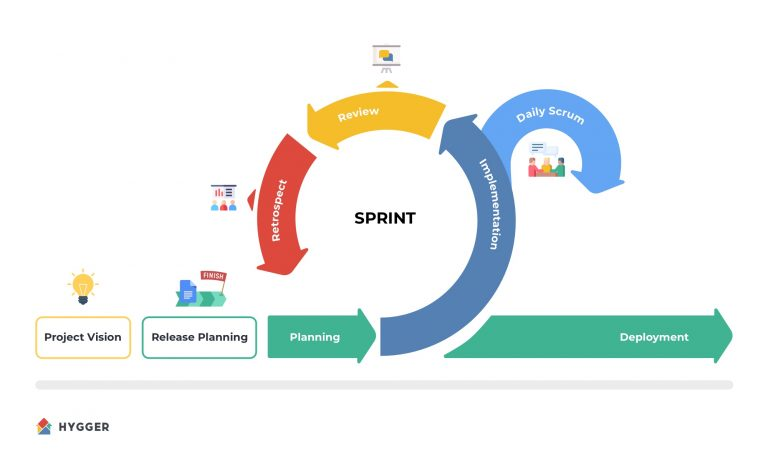
\includegraphics[width=\figwidth]{img/scrum.png}
    \caption{Methodologie Scrum}
    \label{fig:Methodologie Scrum}
\end{figure}

\subsubsection{Méthodologie CRISP-DM}
Processus structuré pour les projets de data mining : Business Understanding, Data Understanding, Data Preparation, Modeling, Evaluation, Deployment.
\begin{figure}[H]
    \centering
    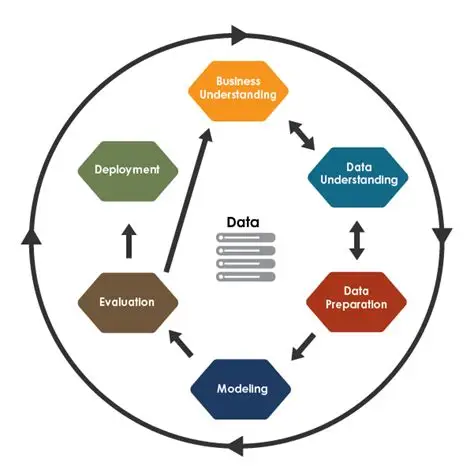
\includegraphics[width=\figwidth]{img/Methodologie CRISP-DM.png}
    \caption{Methodologie CRISP-DM}
    \label{fig:Methodologie CRISP-DM}
\end{figure}

\subsubsection{Combinaison des méthodologies}
Intégration des approches Agile et CRISP-DM pour un développement efficace et structuré.



